\newpage
\section{Общие сведения о системе}
\subsection{Запуск приложения}

\tmis~работает через Web-интерфейс и не требует установки на клиентской рабочей станции никакого дополнительного программного обеспечения. Единственным обязательным условием является наличие установленного Web-браузера, который, как правило, включен по умолчанию в состав любой операционной системы.

Для запуска приложения следует использовать соответствующий ярлык на рабочем столе. При его отсутствии можно запустить Web-браузер и в адресной строке ввести адрес сервера, через который осуществляется доступ к системе. Адрес сервера можно уточнить у администратора системы. 

\subsection{Вход в систему}

После запуска \tmisr , необходимо выполнить вход в систему, используя персональный идентификатор пользователя и пароль. Процедура входа в систему называется \dm{авторизацией}. \label{auth}

Перед первым входом в систему необходимо получить персональный идентификатор пользователя (логин) и пароль у администратора системы.

\begin{vnim}
 Персональный идентификатор и пароль предназначены для индивидуального доступа в систему. Никогда не сообщайте их третьим лицам!
\end{vnim}
 
Следует ввести идентификатор пользователя и пароль в соответствующие поля на странице входа в систему (Рисунок \ref{img_gen_login}) и нажать кнопку \btn{Войти}. 

\begin{figure}[!ht]\centering
 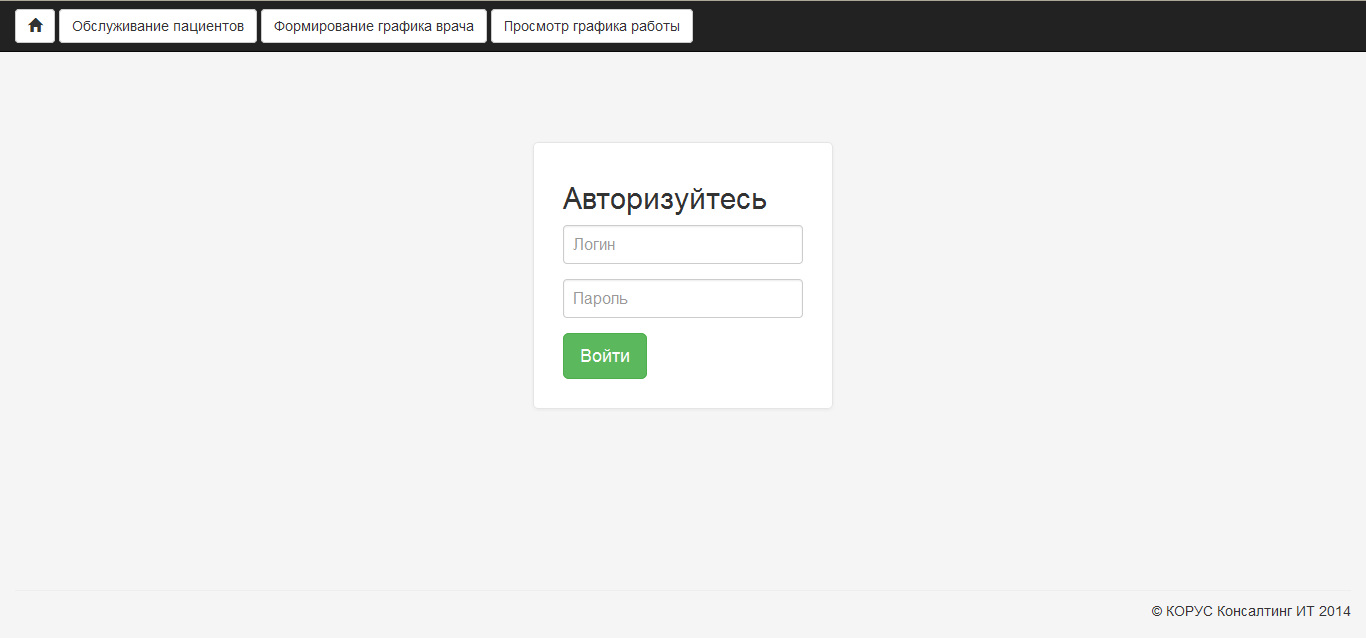
\includegraphics[width = 1\textwidth ,keepaspectratio]{gen_login}
 \caption{Страница авторизации}
 \label{img_gen_login}
\end{figure} 

В случае, если у пользователя имеется несколько ролей, откроется страница выбора роли (Рисунок \ref{img_gen_role}), где  нужно выбрать роль, под которой будет осуществляться работа в текущий момент, из раскрывающегося списка  и нажать кнопку \btn{Выбрать}. В случае, если у пользователя имеется только одна роль, она будет выбрана автоматически. Откроется главная страница системы (Рисунок \ref{img_gen_main}). В зависимости от выбранной роли пользователя и доступных ему функций, внешний вид страницы может отличаться.  

\begin{figure}[!ht]\centering
 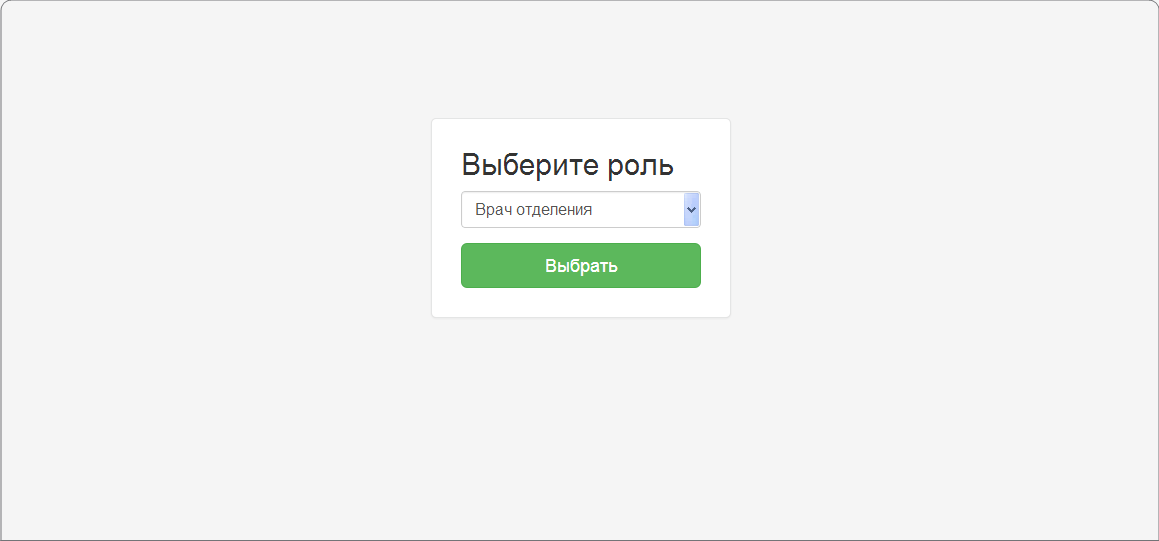
\includegraphics[width = 1\textwidth ,keepaspectratio]{gen_role}
 \caption{Страница выбора роли пользователя}
 \label{img_gen_role}
\end{figure} 

\begin{figure}[!ht]\centering
 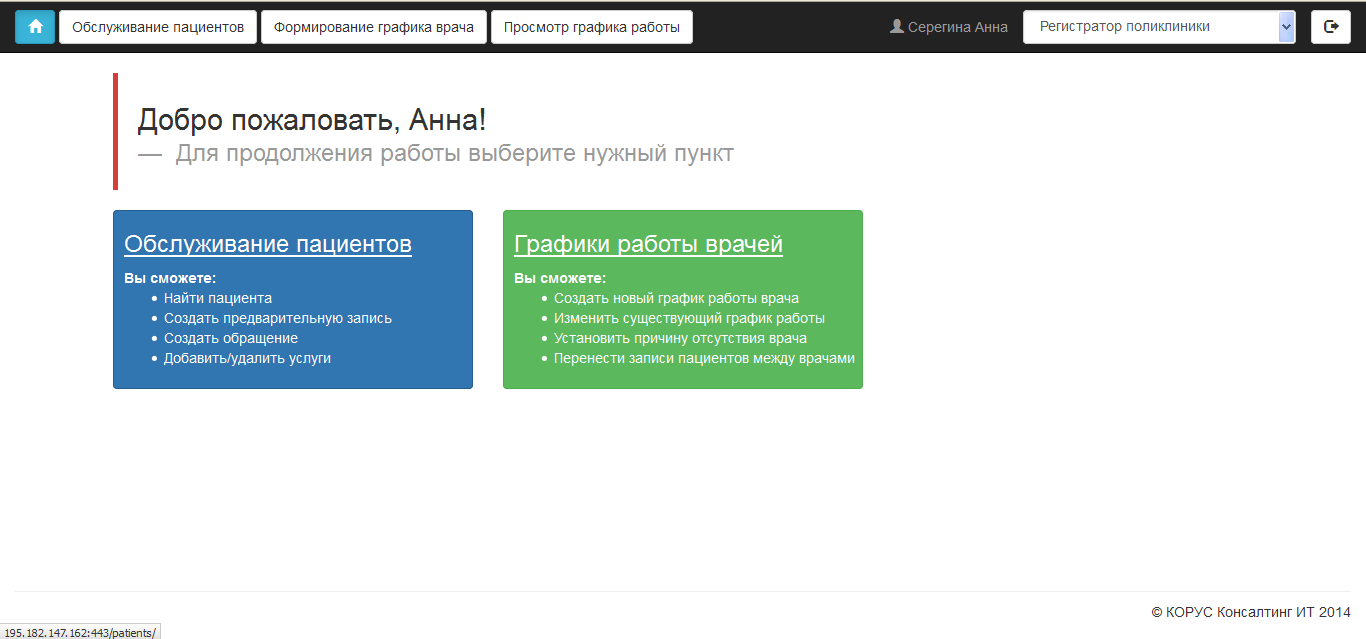
\includegraphics[width = 1\textwidth ,keepaspectratio]{gen_main}
 \caption{Главная страница системы}
 \label{img_gen_main}
\end{figure} 

Если идентификатор пользователя или пароль были введены неверно, то вход в систему не будет осуществлен, а над полем для ввода имени пользователя появится сообщение об ошибке <<Неверное имя пользователя или пароль>> (Рисунок \ref{img_gen_lfail}).

\begin{figure}[!ht]\centering
 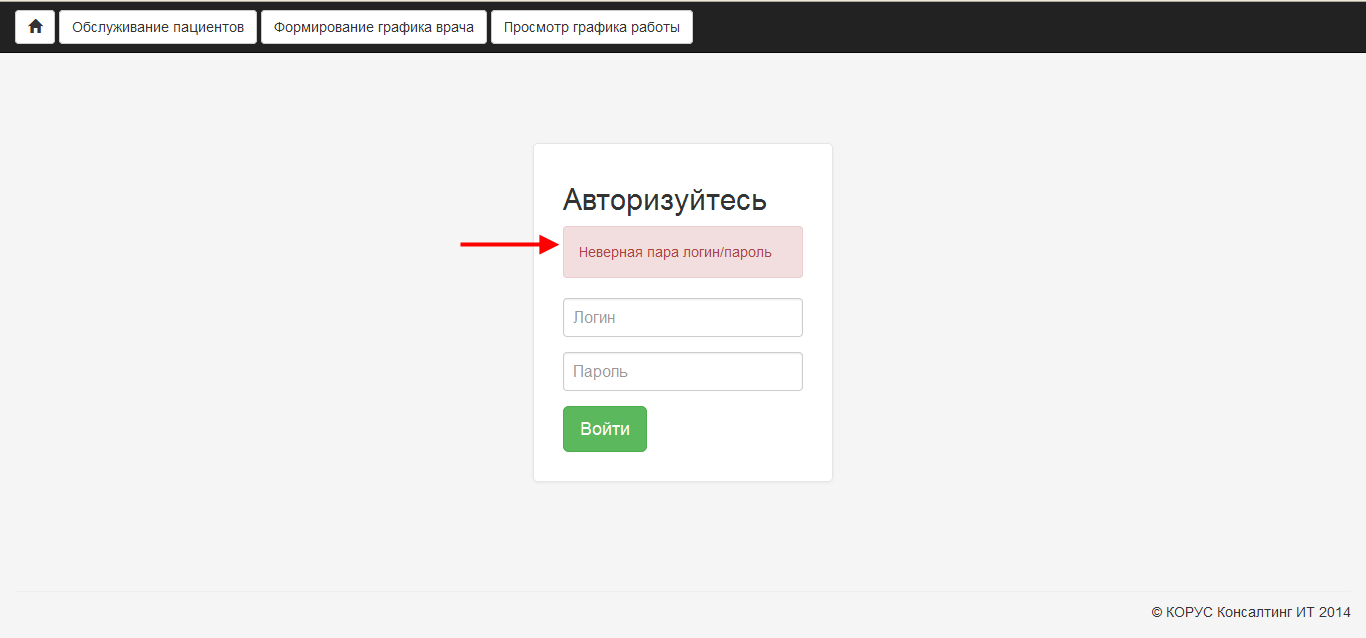
\includegraphics[width = 0.4\textwidth ,keepaspectratio]{gen_lfail}
 \caption{Ошибка авторизации}
 \label{img_gen_lfail}
\end{figure} 

В случае возникновения ошибки необходимо:
\begin{enumerate}
 \item Проверить правильность введенного идентификатора пользователя;
 \item Проверить правильность введенного адреса для подключения (если вводился вручную);
 \item Проверить язык ввода;
 \item Проверить состояние клавиши \keys{CapsLock} на клавиатуре и выключить ее при необходимости;
 \item Если в пароле присутствуют цифры, проверить состояние клавиши \keys{NumLock}, включить ее при необходимости;
 \item Повторить попытку авторизации.
\end{enumerate}
 
Если проблема не была решена, нужно обратиться к администратору системы для проверки идентификационных данных.

\ifthenelse{\isnamedefined{assistversion} \OR \isnamedefined{fullversion}}
{
\subsection{Выбор врача для ассистирования} \label{gen_assist}

В случае входа в систему в качестве медсестры-ассистента врача, перед началом работы следует выбрать врача, которому будет осуществляться ассистирование. Страничка выбора врача открывается автоматически сразу после входа в систему (Рисунок \ref{img_gen_assist_log}). 

 \begin{figure}[!ht]\centering
 	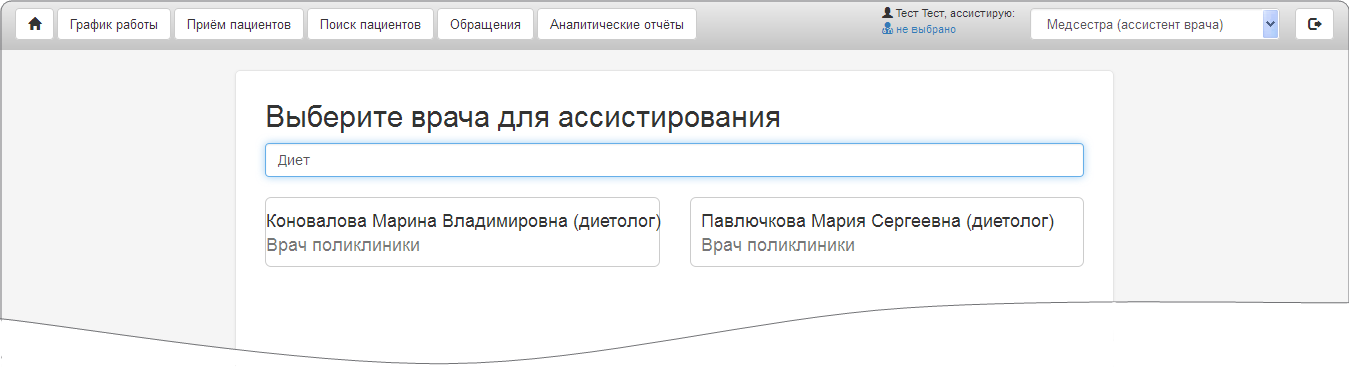
\includegraphics[width = 1\textwidth ,keepaspectratio]{gen_assist_log}
 	\caption{Страница выбора врача для ассистирования}
 	\label{img_gen_assist_log}
 \end{figure} 

В верхней части страницы находится поле поиска \slash фильтрации списка врачей. В данное поле можно ввести часть фамилии или специальность врача. По мере ввода текста в поле, список врачей будет фильтроваться в соответствии с условиями поиска -- в списке останутся только врачи, чья специальность или фамилия содержат введенное буквосочетание. Для возврата к полному списку врачей следует очистить поле поиска. Для перемещения по списку можно использовать полосу прокрутки в правой части списка или колесо мыши.

Когда нужный врач найден в списке, следует щелкнуть по панели с его фамилией и специальностью. Указанный врач будет выбран, и его фамилия появится во всплывающем окне управления профилем пользователя (Рисунок \ref{img_gen_assist_name}). При этом медсестре становятся доступны те же функции, что и выбранному врачу.

 \begin{figure}[!ht]\centering
 	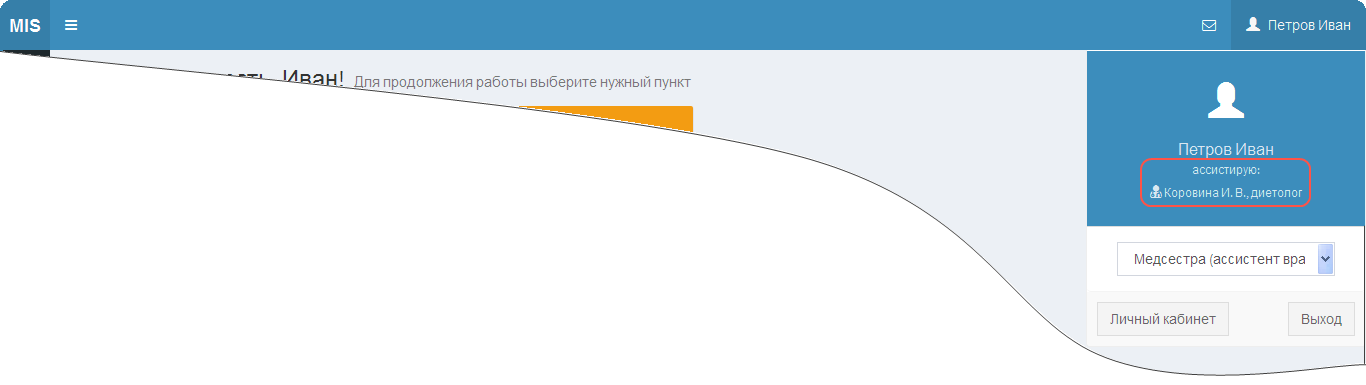
\includegraphics[width = 1\textwidth ,keepaspectratio]{gen_assist_name}
 	\caption{Указание фамилии врача для ассистирования}
 	\label{img_gen_assist_name}
 \end{figure}
}{} 
 
\subsection{Завершение работы} \label{gen_exit}

После окончания работы, необходимо щелкнуть по имени пользователя в правом верхнем углу страницы и в появившемся всплывающем окне нажать кнопку \btn{Выход}.  Будет осуществлен выход из системы и возврат на страницу авторизации. Если требуется войти в систему под другим именем пользователя, следует пройти процедуру авторизации с новыми идентификационными данными. Если работа с системой завершена, можно закрыть Web-браузер, нажав на кнопку \btn{x} в правом верхнем углу окна или выбрав в главном меню пункт \mm{Файл \str Выход}.


\subsection{Основные принципы работы}

Вся работа в системе производится в окне Web-браузера. В верхней части каждой страницы находится панель управления (Рисунок \ref{img_gen_main}), на которой расположены основные управляющие элементы системы. Панель управления отображается на всех страницах \tmisr.  В левом верхнем углу панели управления расположена кнопка \btn{MIS} (при компактном виде панели навигации) или \btn{WebMIS} (при расширенном), при нажатии на которую выполняется переход на главную страницу системы (Рисунок \ref{img_gen_main}). Кнопка 
\includegraphics[scale=0.7]{widemode} позволяет переключать вид панели навигации, расположенного в левой части страницы. Ондократное нажатие на данную кнопку приводит панель навигации к расширенному виду (Рисунок \ref{img_gen_widemenu}), повторное нажатие возвращает к компактному виду, принятому по умолчанию.

 \begin{figure}[!ht]\centering
 	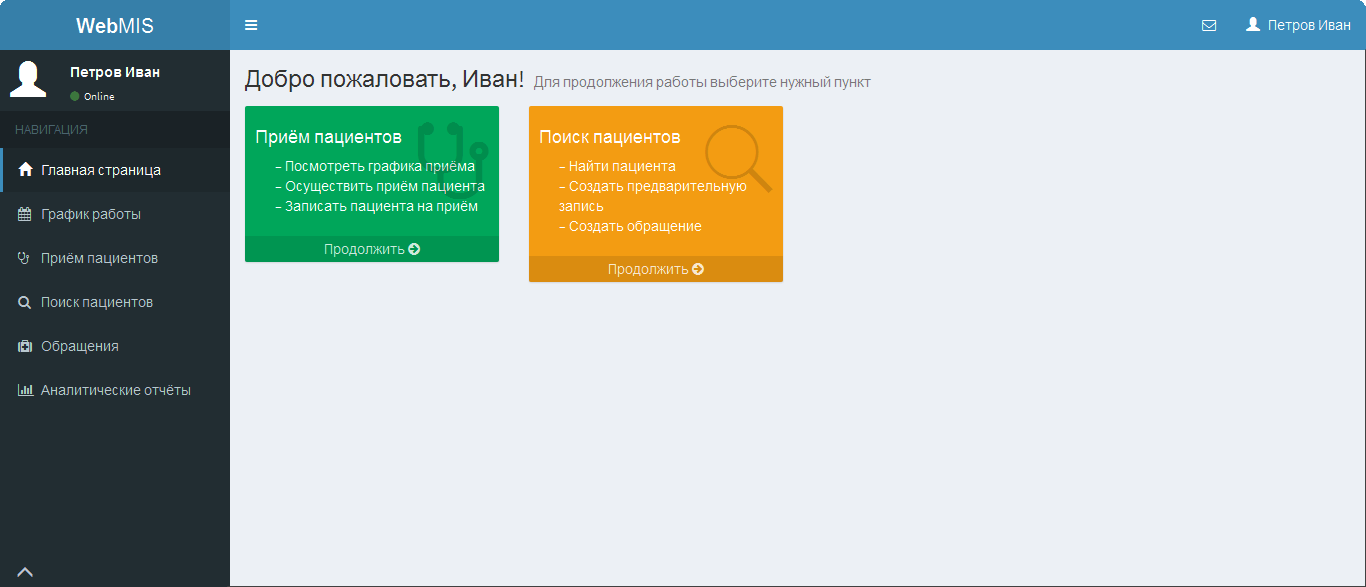
\includegraphics[width = 1\textwidth ,keepaspectratio]{gen_widemenu}
 	\caption{Расширенный вид панели навигации}
 	\label{img_gen_widemenu}
 \end{figure}
 
В правой части панели управления размещаются элементы, позволяющие получить доступ к персональным разделам пользователя: 
\begin{itemize}
 \item внутренняя электронная почта;
 \item персональные настройки пользователя;
 \item управление ролями пользователя.
\end{itemize}

По левому краю страницы находится панель навигации (см. п. \ref{gen_navpanel}). 

\begin{prim}
 После авторизации в \tmisp~возможно одновременное открытие нескольких рабочих страниц системы. Страницы могут быть открыты в отдельных окнах или вкладках. Для открытия страницы в новой вкладке или новом окне можно воспользоваться контекстным меню или колесом прокрутки мыши.
\end{prim}


\subsubsection{Внутренняя электронная почта}

Каждый пользователь системы имеет возможность получения и отправки сообщений другим пользователям, а так же получения системных уведомлений с помощью внутренней электронной почты.

Функциональные возможности и принцип работы внутренней электронной почты аналогичны большинству почтовых клиентов и web-сервисов в сети Internet:
\begin{itemize}
 \item Получение и просмотр электронных писем;
 \item Создание и отправка электронных писем;
 \item Удаление электронных писем;
 \item Пометка важных электронных писем.
\end{itemize}

Однако, внутренняя электронная почта имеет ряд ограничений:
\begin{itemize}
 \item Обмен сообщениями возможен только между пользователями \tmisr;
 \item Отсутствует возможность прикрепления файлов к письму.
\end{itemize}
 
Для перехода к внутреннему почтовому клиенту нужно щелкнуть по кнопке 
\includegraphics[scale=1]{msg} на панели управления. Будет осуществлен переход на страницу \dm{Почтовый ящик} (Рисунок \ref{img_gen_mail_main}). В левой части страницы почтового ящика располагается перечень папок:
\begin{itemize}
 \item \dm{Входящие} -- содержит сообщения, полученные текущим пользователем от других пользователей системы.
 \item \dm{Помеченные} -- содержит сообщения, отмеченные пользователем.
 \item \dm{Отправленные} -- содержит сообщения, отправленные другим пользователям системы.
 \item \dm{Системные} -- сообщения и уведомления, автоматически формируемые системой.
 \item \dm{Корзина} -- сообщения, удаленные пользователем.
\end{itemize}

 \begin{figure}[!ht]\centering
 	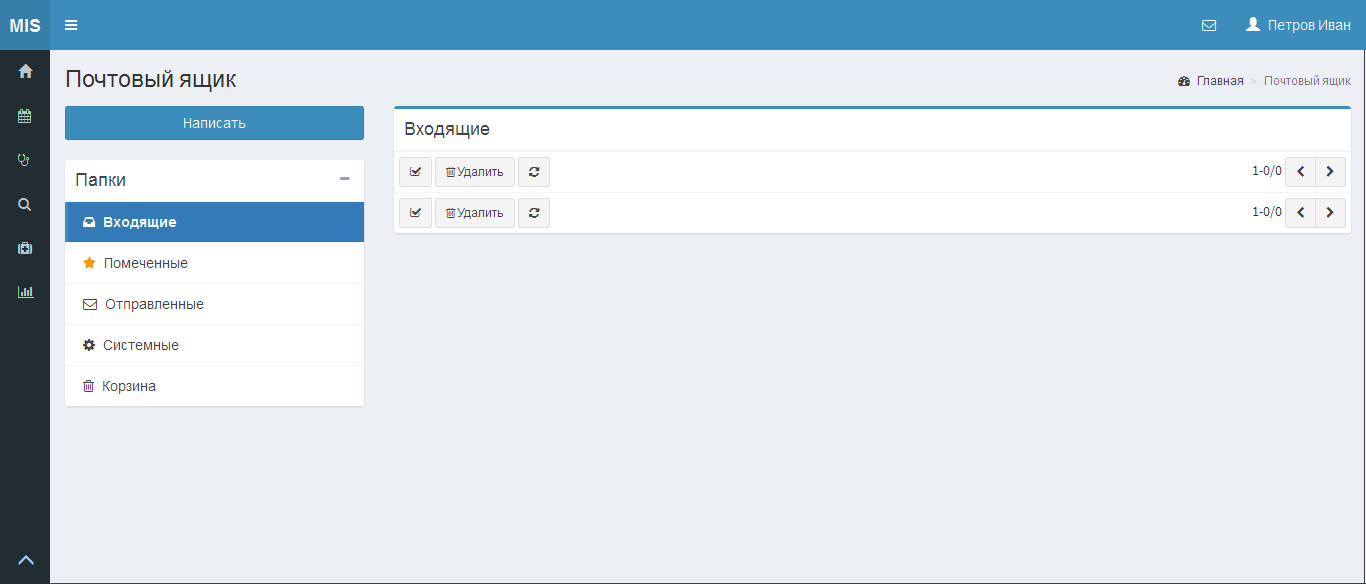
\includegraphics[width = 1\textwidth ,keepaspectratio]{gen_mail_main}
 	\caption{Страница \dm{<<Почтовый ящик>>}}
 	\label{img_gen_mail_main}
 \end{figure}

Щелкнув левой кнопкой мыши по названию соответствующей папки, можно перейти в нее, при этом в основной части страницы появится список писем данной папки. Для каждого письма отображается его отправитель (для полученных) или получатель (для отправленных), тема письма и дата/время отправки. Темы писем, которые еще не были прочитаны пользователем, выделена жирным шрифтом.

Порядок расположения писем в папках осуществлен таким образом, что вначале списка отображаются наиболее новые (по времени отправки) письма. Если в папке содержится достаточно большое количество писем, они могут быть разбиты на страницы. Для перемещения по страницам следует использовать кнопки 
\includegraphics[scale=0.7]{arr_back} и 
\includegraphics[scale=0.7]{arr_next} , расположенные вверху и внизу каждой страницы.

Для создания нового электронного письма нужно нажать кнопку \btn{Написать} в левом верхнем углу страницы и заполнить следующие поля (Рисунок \ref{img_gen_mail_new}):
\begin{enumerate}
 \item \dm{Кому} -- имя получателя выбирается из справочника пользователей системы. Нужно ввести часть фамилии или специальности врача в данное поле, а затем выбрать нужное значение в появившемся списке. Для сообщения возможно указать только одного получателя. 
 \item \dm{Тема} -- тема(заголовок) письма.
 \item Текст письма произвольной длины. В данном поле возможно форматирование текста: выбор стиля и размера шрифта, добавление отступов, создание маркированных и нумерованных списков и т.д.
\end{enumerate}

Все перечисленные поля являются обязательными для заполнения. После их заполнения становится активной кнопка \btn{Отправить}, которую необходимо нажать после того, как сообщение полностью сформировано, для его отправки получателю. Все отправленные письма сохраняются в папке \dm{Отправленные}.
  
 \begin{figure}[!ht]\centering
 	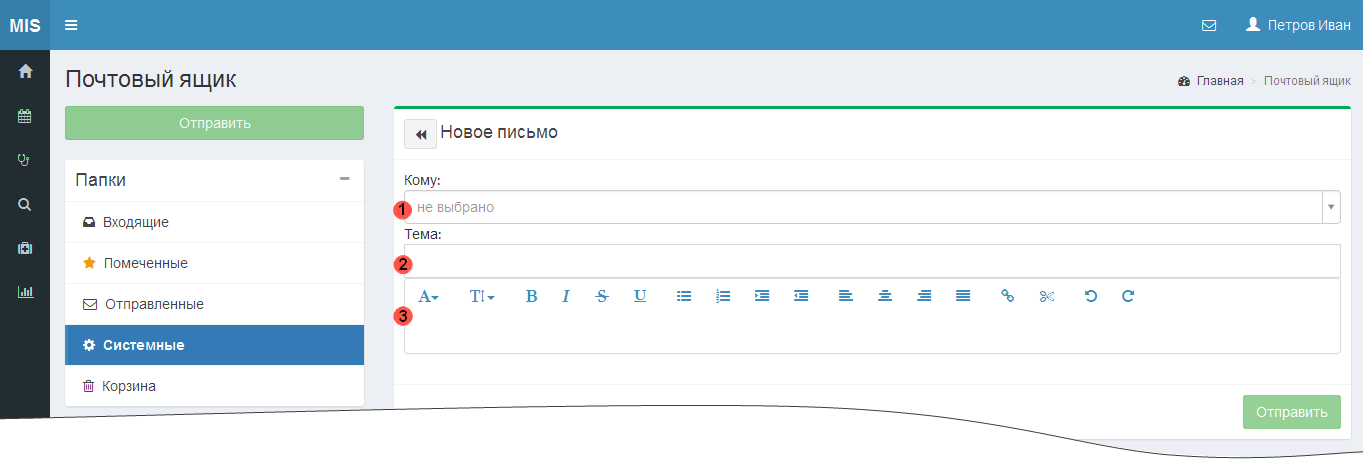
\includegraphics[width = 1\textwidth ,keepaspectratio]{gen_mail_new}
 	\caption{Создание нового электронного сообщения}
 	\label{img_gen_mail_new}
 \end{figure}

Для удаления писем из папки нужно установить флажок напротив одного или нескольких сообщений, подлежащих удалению, и нажать кнопку \btn{Удалить} вверху или внизу списка. После непродолжительного ожидания, отмеченные сообщения исчезнут с экрана. Удаленные сообщения можно найти в папке \dm{Корзина}.

Электронные письма из папок \dm{Входящие} и \dm{Системные} могут быть помечены, как важные. Для этого нужно щелкнуть левой кнопкой мыши по звездочке слева от темы соответствующего письма. При этом звездочка окрасится в желтый цвет, а письмо стнет отображаться в папке \dm{Помеченные}.

Проверка и получение новых электронных писем выполняется с заданной периодичностью. Для проверки почты и получения новых писем в текущий момент можно воспользоваться кнопкой 
\includegraphics[scale=0.7]{refresh}, расположенной в каждой папке вверху и внизу списка писем.

\ifthenelse{\isnamedefined{assistversion} \OR \isnamedefined{fullversion}}
{
\begin{vnim}
Сообщения внутренней электронной почты доступны только персонально пользователю. Медсестре в роли ассистента врача НЕ доступны личные сообщения врача, которому она ассистирует.
\end{vnim}
}{}

\subsubsection{Персональное меню пользователя}

В правом верхнем углу рабочего окна, на панели управления, указано имя пользователя, под которым осуществлен вход в систему в данный момент. Щелкнув по нему левой кнопкой мыши, можно раскрыть персональное меню пользователя (Рисунок \ref{img_gen_assist_name}). В данном меню доступны следующие функции:

\begin{itemize}
 \item Просмотр и смена текущей роли пользователя;
 \ifthenelse{\isnamedefined{assistversion} \OR \isnamedefined{fullversion}}
 {
 \item Просмотр и смена врача, которому выполняется ассистирование;
 }{}
 \item Переход к персональному разделу пользователя;
 \item Выход из системы.
\end{itemize}

Текущая роль, под которой работает пользователь указана в поле раскрывающегося списка в персональном меню пользователя (Рисунок \ref{img_gen_assist_name}). Если пользователю доступно несколько ролей в системе, то для изменения текущей роли достаточно выбрать ее в раскрывающемся списке. Права доступа и список функций пользователя немедленно будет обновлен в соответствии со вновь выбранной ролью. 

\ifthenelse{\isnamedefined{assistversion} \OR \isnamedefined{fullversion}}
{Просмотр и смена врача, которому выполняется ассистирование, подробно описано в подразделе \ref{gen_assist}
}{}


Щелкнув левой кнопкой мыши по кнопке \btn{Личный кабинет} можно перейти к персональному разделу пользователя, где в зависимости от административных настроек конкретного ЛПУ доступны:

\begin{itemize}
 \item внутренняя электронная почта пользователя;
 \item персональные визуальные настройки рабочих окон системы.
\end{itemize}

Завершение работы с системой подробно описано в подразделе \ref{gen_exit}

\subsubsection{Панель навигации} \label{gen_navpanel}

По левому краю каждой страницы располагается панель навигации пользователя, обеспечивающая доступ ко всем функциям системы. В зависимости от выбранной роли пользователя в системе, состав ссылок панели навигации может быть различен. Панель навигации  может отображаться в компактном (по умолчанию) (Рисунок \ref{img_gen_main}) или расширенном виде (Рисунок \ref{img_gen_widemenu}). Переключение внешнего вида осуществляется кнопкой 
\includegraphics[scale=0.7]{widemode}, расположенной в левой части панели управления.

В компактном виде ссылки отображаются в виде пиктограмм. При наведении на пиктограмму указателя мыши, появляется подсказка, содержащяя название функции. Щелчок левой кнопки мыши по пиктограмме позволяет перейти к странице работы с выбранной функцией системы. Компактный вид панели навигации занимает минимальное место на экране, что оставляет больше пространства для рабочей области. 

В расширенном виде панели навигации ссылки отображаются в виде сочетания пиктограммы и названия функции. Для перехода к работе с выбранной функцией, необходимо щелкнуть левой кнопкой мыши по соответствующей ссылке.

\subsubsection{Главная страница}

Сразу после входа в систему открывается главная страница \tmisr~(Рисунок \ref{img_gen_main}). В зависимости от роли пользователя в системе на данной странице содержится одна или несполько плиток, описывающих основные доступные для текущей роли пользователя функции. Щелкнув левой кнопкой мыши по ссылке \dm{Продолжить} или непосредственно по плитке, можно перейти к странице работы с выбранной функцией. 

Вызов главной страницы так же возможен в любой момент времени с панели навигации щелчком левой кнопки мыши по соответствующей пиктограмме или нажатием кнопки \btn{MIS} $\backslash$ \btn{WebMIS} в левом верхнем углу страницы.


\subsubsection{Поиск и фильтрация данных в справочниках} \label{gen_filtr}

Большинство справочников в \tmisr~предоставляют возможности поиска и фильтрации данных.

\dm{Фильтрация} -- выбор и отображение только тех данных, которые удовлетворяют критериям поиска.

Фильтрация данных организована одинаково практически во всех справочниках системы. Если в каком-либо из справочников используется механизм фильтрации, отличный от стандартного, это будет отмечено при описании соответствующего раздела. Стандартный же механизм фильтрации заключается в следующем:
\begin{itemize}
 \item При раскрытии справочника в верхней или нижней его части (в зависимости от местоположения справочника на странице) появляется поле для задания строки поиска (Рисунок \ref{img_gen_filtr}). Справа оно помечено значком 
\includegraphics[scale=0.7]{filtr}.
 
 \begin{figure}[!ht]\centering
 	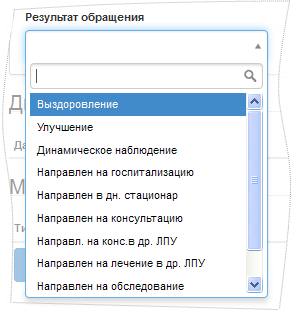
\includegraphics[width = 0.4\textwidth ,keepaspectratio]{gen_filtr}
 	\caption{Поле поиска \slash фильтрации данных справочника}
 	\label{img_gen_filtr}
 \end{figure} 
 
 \item При раскрытии справочника курсор автоматически помещается в поле поиска. Можно сразу начинать ввод строки поиска.
 \item Фильтрация производится по мере ввода текста в поле поиска. Т.е. состав элементов справочника меняется при вводе каждого нового символа в поле поиска. Нажатия дополнительных кнопок для запуска поиска не требуется.
 \item В результаты поиска попадают записи, содержащие введенный текст. Текст может находиться в любом месте записи (не обязательно в начале наименования или слова).
 \item Регистр букв не учитывается при поиске.
 \item В активной записи найденная подстрока выделется цветом (Рисунок \ref{img_gen_filtr2}).
 \item Для отмены фильтрации и получения полного справочника следует очистить поле поиска.
\end{itemize} 

\begin{figure}[!ht]\centering
	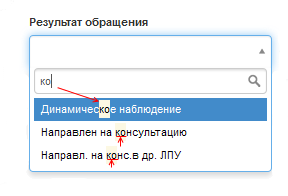
\includegraphics[width = 0.4\textwidth ,keepaspectratio]{gen_filtr2}
	\caption{Применение фильтрации данных}
	\label{img_gen_filtr2}
\end{figure}  

\subsubsection{Работа с элементом управления <<Календарь>>} \label{gen_cal}

Элемент управления <<Календарь>> используется во всех полях, содержащих дату, в системе. На некоторых страницах (например, при работе с расписанием) он находится постоянно в раскрытом виде, в других случаях раскрывается по нажатию кнопки 
\includegraphics[scale=0.7]{cal} справа от соответствующего поля либо установке курсора в поле для ввода даты. Во всех случаях принцип работы с календарем одинаков.

Для выбора даты из календаря, достаточно щелкнуть по нужному числу месяца в календаре левой кнопкой мыши.  Как правило, по умолчанию в календаре открывается текущий месяц и выбирается текущий день. Если в поле размещения календаря уже введена какая-то дата, то календарь открывается на месяце указанного года, к которому относится дата. Если календарь привязан к полю ввода даты, то можно ввести дату с клавиатуры (достаточно ввести только цифры, без разделителей). Разделители будут подставлены автоматически в соответствии с форматом даты. При этом в календаре будет автоматически выбрана введенная дата.

Для перехода по месяцам можно использовать стрелки, расположенные справа и слева от названия месяца в верхней части календаря (Рисунок \ref{img_gen_caldrill}). При нажатии на стрелки будет осуществляться переход к следующему или предыдущему месяцу соответственно.

\begin{figure}[!ht]\centering
	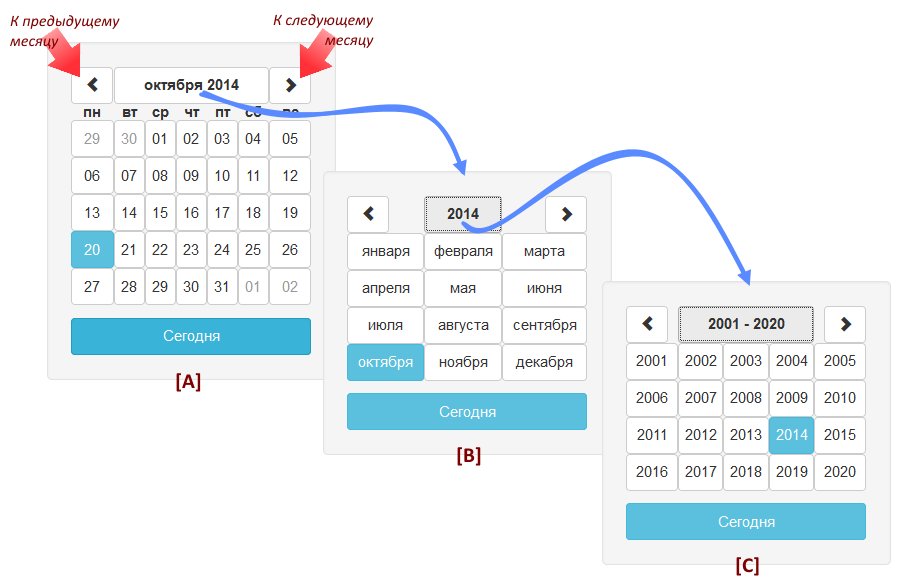
\includegraphics[width = 0.8\textwidth ,keepaspectratio]{gen_caldrill}
	\caption{Механизм работы календаря}
	\label{img_gen_caldrill}
\end{figure} 

Можно выбрать произвольный месяц из календаря. Для этого следует нажать на кнопку с названием месяца в верхней части календаря. После этого календарь примет вид [B] (Рисунок \ref{img_gen_caldrill}). В верхней части календаря будет указан номер года. Стрелки, расположенные слева и справа от номера года, позволяют перейти к предыдущему или следующему году. Щелчок левой кнопкой мыши по названию месяца позволяет раскрыть числа этого месяца.

При нажатии на кнопку с номером года в верхней части календаря, он примет вид [C] (Рисунок \ref{img_gen_caldrill}). В основной части календаря будут отображаться номера лет текущего двадцатилетия. Переход к следующему или предыдущему двадцатилетию осуществляется при нажатии на кнопки, расположенные слева и справа от кнопки, содержащей интервалы лет. При нажатии на кнопку с интервалами лет осуществляется возврат к текущему месяцу (вид [A]). Для выбора даты в календаре вида С следует щелкнуть левой кнопкой мыши по номеру нужного года, далее в видоизменившемся календаре вида В выбрать месяц, и затем - число месяца.
 
Для быстрого возврата к просмотру текущего дня либо установки текущей даты в поле ввода предусмотрена кнопка \btn{Сегодня} в нижней части календаря. 

При раскрытии календаря в поле ввода в нем появляются так же дополнительные кнопки:

\begin{itemize}
	\item \btn{Недели} -- позволяет скрывать и отображать номера недель в крайнем левом столбце календаря. Кнопка работает по принципу переключателя: если первое нажатие скрывает номера недель, то повторное - снова их отображает.
	\item \btn{Убрать} -- скрывает календарь и очищает поле ввода даты.
	\item \btn{Готово} -- скрывает календарь, сохраняя при этом введенное в поле значение. 
\end{itemize}